% Preamble
% --------
\documentclass[12pt]{article}

\newcommand{\codename}[0]{\texttt{apex-sim}~}

% Packages
% --------
\usepackage{blindtext} %for boilerplate text (\blindtext)
\usepackage{geometry} %for paper dimensions and margins
\usepackage{graphicx} % for including graphics
\usepackage{hyperref} % for hyperlink support

% Page Setup
% ----------
\geometry{letterpaper, margin=1in}

% Title content and formatting
% ----------------------------
\title{Apex Instruction Set Architecture Simulator (\texttt{apex-sim}) \\ Phase 1 Documentation}
\author{Matthew Cole \\ \texttt{mcole8@binghamton.edu}
\and
Brian Gracin \\ 
	\texttt{bgracin1@binghamton.edu}}
\date{19 November 2016}

\begin{document}
% Emit title content
% ------------------
\pagenumbering{gobble}
\maketitle
\tableofcontents
\listoffigures
\newpage
\pagenumbering{arabic}

%%%%%%%%%%%%%%%%%%%%%%%%%%%%%%%%%%%%%%%%%%%%%%%%%%%%%%%
\section{Design}
\codename is a simulator for the \textit{Architecture Pipeline EXample} (APEX) Instruction Set Architecture (ISA).
\codename consists of the following components:
\begin{itemize}
  \item \texttt{main.cpp} contains the driver program. The driver program provides file input for instructions, user interface operations, and maintaining persistent simulator state. This component is discussed in section \ref{sec:driver}.
  \item \texttt{code.cpp}, \texttt{data.cpp}, \texttt{registers.cpp}, \texttt{cpu.cpp}, and \texttt{stage.cpp} provide the objects modeling components of the pipeline. These components are discussed in section \ref{sec:classes}.
  \item \texttt{simulate.cpp} provides the functions that allow the CPU to simulate working on each of its stages, inter-stage communication through advancement, stalls for basic inter-stage interlocks, and forwarding. These implementation details are described in section \ref{sec:implementation}.
\end{itemize}
Figure \ref{fig:overview} shows class interactions and data flow between each of the stages and support classes.
Finally, we opensource our work under the MIT license through a GitHub repository located at \url{https://github.com/colematt/apex-sim}. We discuss our team's work log in section \ref{sec:production}.

\begin{figure}
  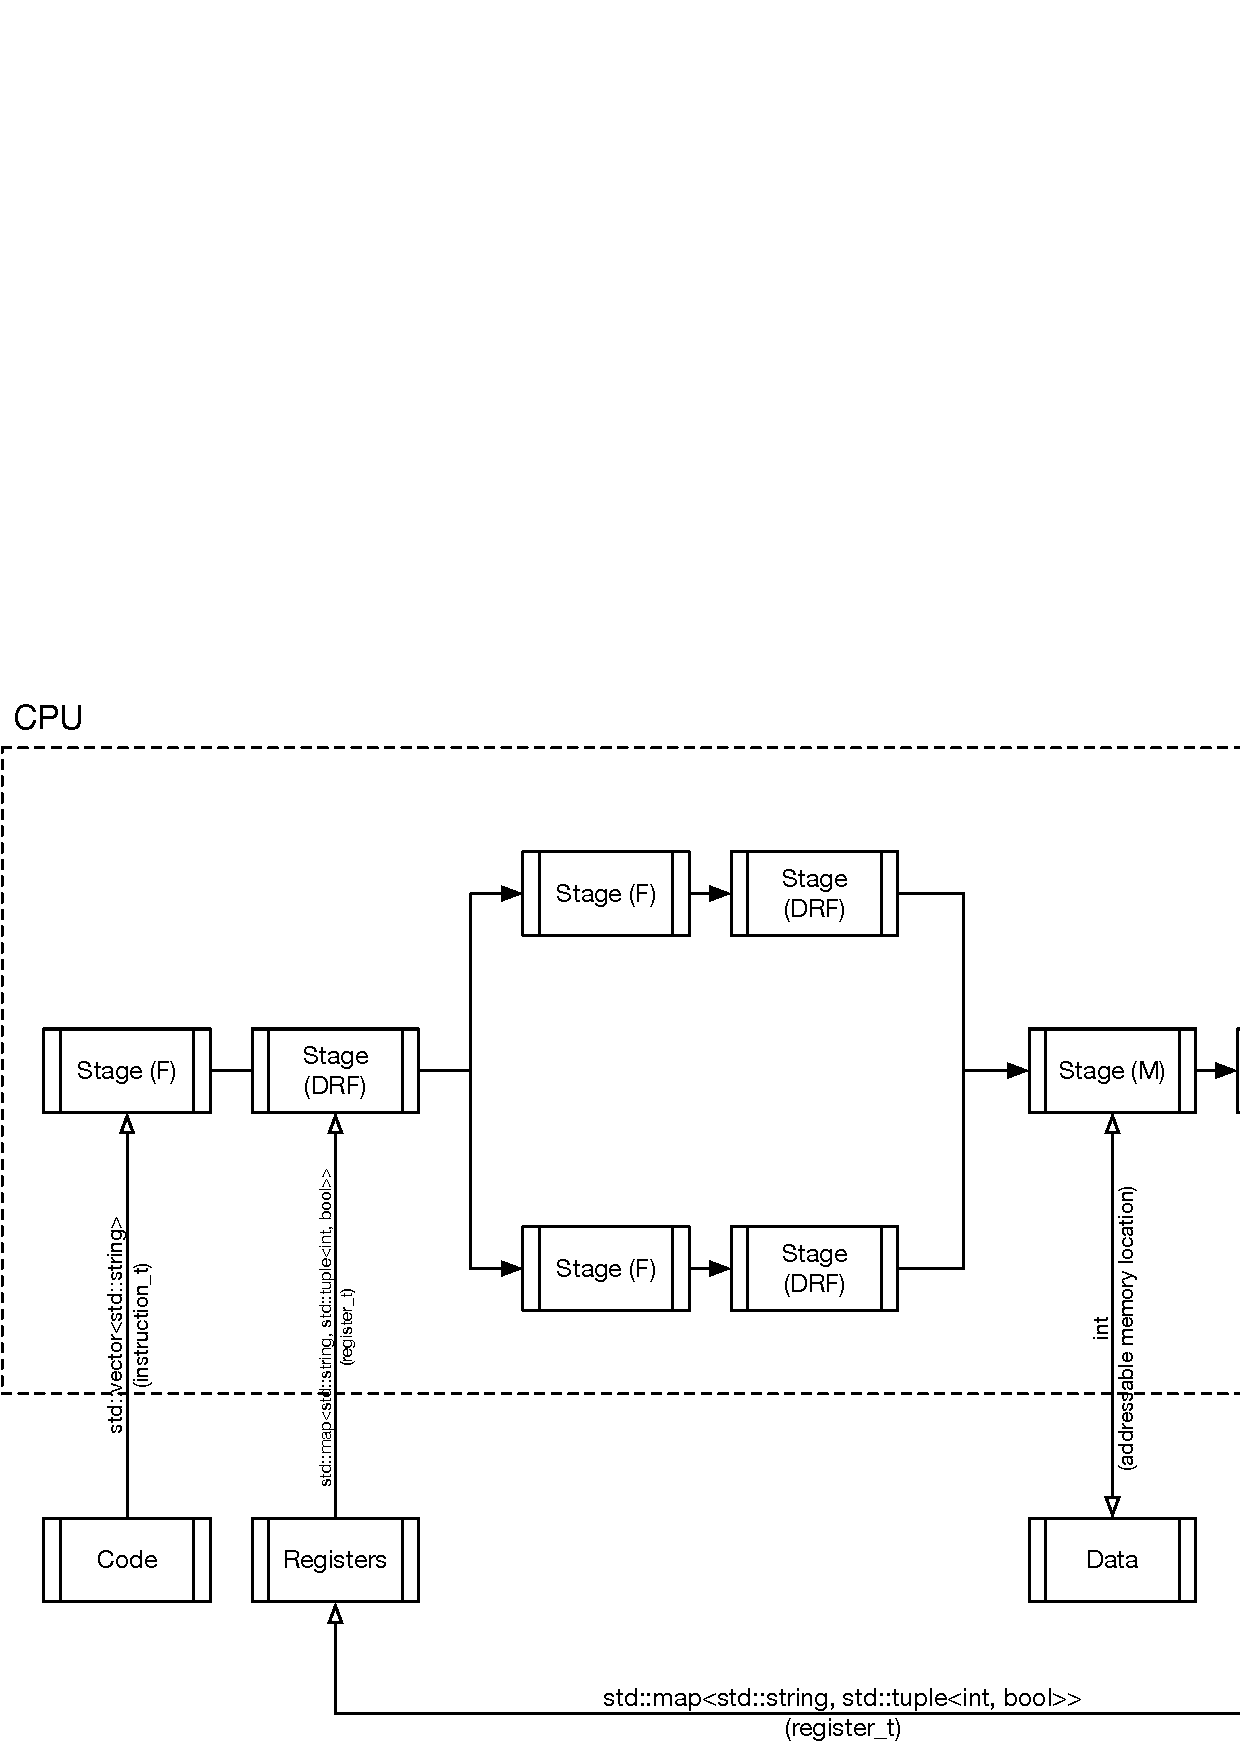
\includegraphics[width=\linewidth]{./figs/apex-sim-overview.pdf}
  \caption{The APEX pipeline and class interactions.}
  \label{fig:overview}
\end{figure}

\subsection{Driver Program}
\label{sec:driver}
The \codename entry point file is \texttt{main.cpp}. This program shepherds execution through the lifecycle of the program and provides a user interface for interacting with the simulator.

\subsection{Classes}
\label{sec:classes}

\subsubsection{Code}

\subsubsection{Data}

\subsubsection{Registers}

\subsubsection{CPU}

\subsubsection{Stages}

%%%%%%%%%%%%%%%%%%%%%%%%%%%%%%%%%%%%%%%%%%%%%%%%%%%%%%%
\section{Implementation}
\label{sec:implementation}

\subsection{Work Phase}

\subsection{Advance Phase}

\subsection{Stalls}

\subsection{Forwarding}


%%%%%%%%%%%%%%%%%%%%%%%%%%%%%%%%%%%%%%%%%%%%%%%%%%%%%%%
\section{Production}
\label{sec:production}

\end{document}


